\documentclass[11pt]{article}
\usepackage[margin=1in]{geometry}
\usepackage{amsmath,amssymb,graphicx,booktabs,array}
\usepackage{hyperref}
\usepackage{listings}
\usepackage{xcolor}

\hypersetup{colorlinks=true,linkcolor=blue,urlcolor=blue}
\lstset{
  basicstyle=\ttfamily\small,
  breaklines=true,
  columns=fullflexible,
  keepspaces=true,
  backgroundcolor=\color{gray!8},
  frame=single,
  framerule=0.2pt,
  xleftmargin=0.5em,
  xrightmargin=0.5em,
}
\graphicspath{{../results/figures/eval/}}

\title{Paper Walkthrough:\\Algorithms, Math, and Implementation}
\author{Learning companion to \texttt{paper/main.tex}}
\date{August 2026}

\begin{document}
\maketitle

\begin{abstract}
This note maps each section of the paper onto the code, spells out the math
the way it is \emph{implemented} (including simplifications), and explains
the Universe~A test results (2020--2025, five seeds).
Figures live under \path{results/figures/eval/}
(regenerate with \texttt{python scripts/run\_eval\_plots.py}).
Pipeline overview: \path{implementation_summary.md}.

\textbf{One-sentence thesis.}
On this long-only, cost-aware MDP, a flat $1/N$ book is so strong that
Decision Transformer matches Behavior Cloning and neither beats buy-and-hold
on Sharpe; RTG conditioning is unused.
\end{abstract}

\tableofcontents
\newpage

\section{Shared MDP (every algorithm)}
\label{sec:mdp}

File: \path{src/env.py}.

Daily rebalancing is the finite-horizon MDP
\[
\mathcal{M}=\langle\mathcal{S},\mathcal{A},P,R,\gamma,\rho_0,T_{\mathrm{ep}}\rangle.
\]
Prices $\{y_t\}$ are \emph{exogenous}: the agent cannot change tomorrow's market.

\begin{center}
\small
\begin{tabular}{@{}llp{0.42\textwidth}@{}}
\toprule
Symbol & Meaning & Code \\
\midrule
$N=14$
  & Investable assets (Universe~A), including cash + synthetic 10Y
  & \texttt{UNIVERSE\_A\_ASSETS} in \path{src/data_loader.py} \\
$y_t$
  & Gross relative returns $p_t/p_{t-1}$
  & \texttt{compute\_price\_returns} \\
$a_t=w_t\in\Delta^{N-1}$
  & Long-only weights, $\sum_i w_i=1$, $w_i\ge 0$
  & softmax / Dirichlet mean / Duchi projection \\
$s_t\in\mathbb{R}^{2580}$
  & Flattened 20-day lookback of returns, technicals, macro, events.
    \emph{Not} previous weights
  & \path{src/features.py} \\
$R_t$
  & $\ln\max(a_t^\top y_t-\mu\|a_t-a_{t-1}\|_1,\varepsilon)$
  & \texttt{compute\_log\_reward}, $\mu=0.001$, $\varepsilon=10^{-8}$ \\
$\gamma$
  & $1$ for DT/RTG; $0.99$ inside value-based RL
  & --- \\
$T_{\mathrm{ep}}$
  & 252 days in training episodes; full split at eval
  & \texttt{env.episode\_length} \\
\bottomrule
\end{tabular}
\end{center}

\paragraph{Turnover caveat.}
The env stores the last \emph{target} $a_{t-1}$, not mark-to-market holdings
$w'\propto a_{t-1}\odot y_t$. Buy-and-hold and equal-weight are therefore the
\textbf{same policy} in this MDP (both always emit $1/N$, so
$\|a_t-a_{t-1}\|_1=0$).

\paragraph{Simplex projection (Duchi 2008).}
Used by MVO/min-var and as a safety net on RL actions:
\begin{equation}
\theta=\frac{\sum_{j=1}^{\rho}u_{(j)}-1}{\rho},\qquad
w=\max(v-\theta,0),\quad w\leftarrow w/\|w\|_1,
\end{equation}
where $u$ is $v$ sorted descending and $\rho$ is the largest index with
$u_i > (\sum_{j\le i}u_j-1)/i$. Batched in \texttt{project\_to\_simplex\_batch}.

\paragraph{Offline data.}
18 behavior policies $\times$ 200 windows $=$ 3{,}600 episodes
(format v2 in \path{src/trajectories.py}).
Shared global \texttt{states} matrix; per-episode \texttt{actions},
\texttt{rewards}, \texttt{rtg}.

\section{Pipeline and architecture choices}
\label{sec:pipeline}

\begin{lstlisting}
prepare -> features -> trajectories -> train (8 algos x 5 seeds) -> evaluate
\end{lstlisting}

\begin{center}
\small
\begin{tabular}{@{}p{0.38\textwidth}p{0.54\textwidth}@{}}
\toprule
Choice & Why \\
\midrule
Causal GPT, not HF transformers
  & Small custom model; full control of the $(\hat R,s,a)$ interleaving
    and padding mask \\
Softmax (or Dirichlet) on the head
  & Hard simplex; no Lagrange multipliers at inference \\
MSE on \textbf{last} context step only
  & Matches Decision Transformer practice; cheaper than summing over $K$ \\
\texttt{steps\_per\_epoch: 200}, batch 256
  & GTX~1070 saturates at $\sim$1{,}300 samples/s; a full pass is
    $\sim$10\,min/epoch ($\sim$87\,h for two transformers $\times$ 5 seeds
    $\times$ 50 epochs). $200\times 256\times 50\approx 3$ passes over the
    816k training samples \\
No AMP
  & Pascal (compute 6.1) has no tensor cores; fp16 would likely slow training \\
\texttt{last\_state\_only} for RL
  & MLP agents do not need the $K$-token gather \\
5 seeds
  & Report mean $\pm$ std; paper tables use this \\
\bottomrule
\end{tabular}
\end{center}

Training loop: \path{src/trainer.py}.
Inference wrappers: \path{src/eval/model_policy.py}
(\texttt{DTPolicy}, \texttt{AgentPolicy}).

\begin{figure}[ht]
\centering
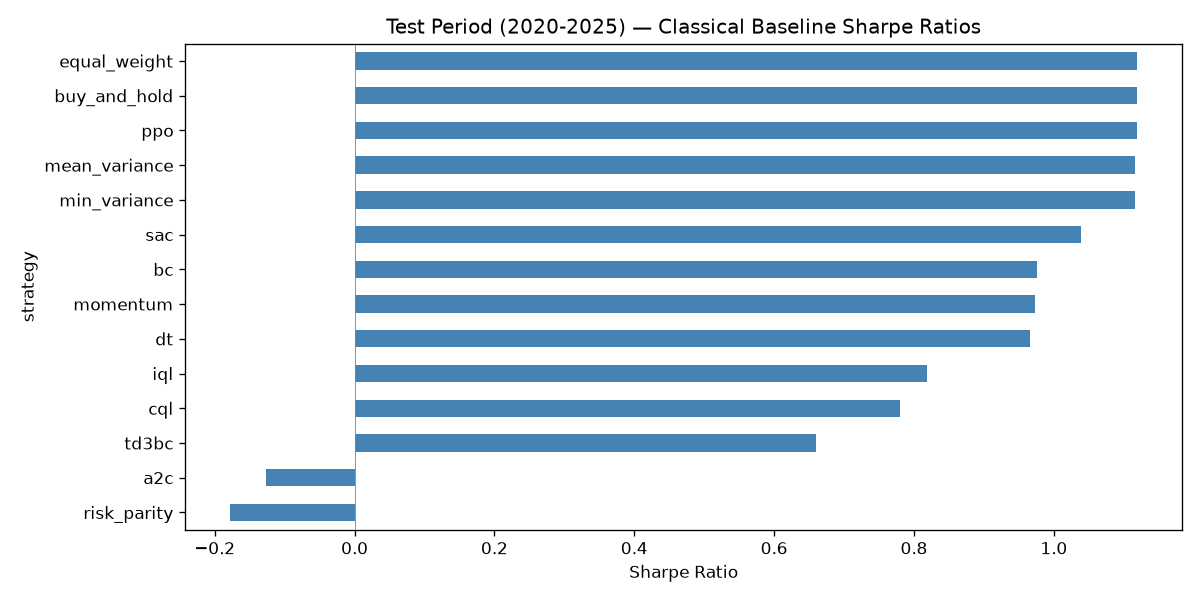
\includegraphics[width=0.92\textwidth]{sharpe_comparison.png}
\caption{Test-period Sharpe (classical + learned means).}
\end{figure}

\begin{figure}[ht]
\centering
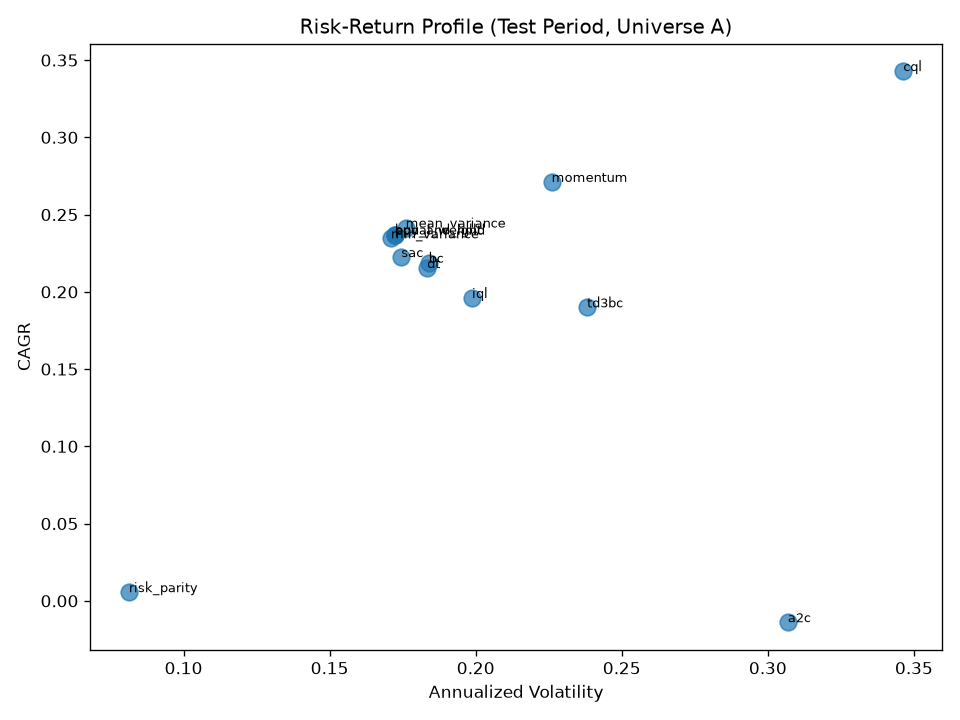
\includegraphics[width=0.92\textwidth]{risk_return_scatter.png}
\caption{Risk--return scatter (CAGR vs.\ volatility).}
\end{figure}

\section{Classical algorithms}
\label{sec:classical}

All live in \path{src/policies.py}. They ignore $s_t$ and use only trailing $y$.
Test window: 2020--2025.

\subsection{Buy-and-hold and equal-weight}

\paragraph{Math.} $a_t=\mathbf{1}/N$ for all $t$.

\paragraph{Implementation.}
\texttt{BuyAndHold} and \texttt{EqualWeight} both copy a cached uniform vector.
Under target-based turnover they produce identical backtests
(Sharpe $1.118$, CAGR $23.7\%$, max DD $-23.3\%$, turnover $\sim 0$).

\paragraph{How to read the result.}
This is the bar every learned method failed to clear on Sharpe.
It is \emph{not} a drifted buy-and-hold (weights never ride winners).

\subsection{Momentum}

\paragraph{Math.}
Lookback $L=60$, top-$k$ with $k=\lfloor N/3\rfloor=4$:
\begin{equation}
c_{i,t}=\prod_{\ell=1}^{L} y_{t-\ell,i}-1,\qquad
a_{i,t}=\frac{1}{k}\mathbf{1}\bigl[i\in\mathrm{arg\,top}_k\,c_{\cdot,t}\bigr].
\end{equation}
If $t<L$, fall back to $1/N$.

\paragraph{Implementation.}
\texttt{Momentum.\_\_call\_\_} / \texttt{precompute}.
Schedules cached in \path{data/processed/policy_weights.npz}.

\paragraph{Result.}
Best CAGR $27.1\%$, Sharpe $0.97$, max DD $-32.0\%$, mean daily turnover $15.1\%$.
Wins 2020--2021 walk-forward, loses 2022--2023.
High turnover is the cost of rotating the top-4 book every day.

\subsection{Mean-variance (max-Sharpe)}

\paragraph{Math.}
On a 252-day window, Ledoit--Wolf $\hat\Sigma$, sample mean $\hat\mu$.
Projected gradient on the simplex ($200$ steps, $\eta=0.05$):
\begin{equation}
w\leftarrow \Pi_{\Delta}\bigl(w-\eta(\hat\mu-\hat\Sigma w)\bigr).
\end{equation}
The gradient of $w^\top\mu-\tfrac12 w^\top\Sigma w$ is $\mu-\Sigma w$.

\paragraph{Implementation.}
\texttt{\_optimize\_weights\_batch} + \texttt{MeanVariance}.
Fallback $1/N$ until the window is full.

\paragraph{Result.}
CAGR $24.2\%$, Sharpe $1.116$ --- statistically the same as $1/N$
(bootstrap CI on Sharpe difference covers 0).
Ledoit--Wolf + simplex projection mostly recovers a near-static book,
hence turnover only $0.7\%$.

\subsection{Min-variance}

\paragraph{Math.}
Same machinery, gradient $2\hat\Sigma w$ (minimize $w^\top\Sigma w$).

\paragraph{Result.}
CAGR $23.5\%$, Sharpe $1.116$, turnover $\approx 0$.
Again indistinguishable from $1/N$ on this universe and window.

\subsection{Risk parity (inverse-vol)}

\paragraph{Math.}
Lookback 60:
\begin{equation}
a_{i,t}\propto \frac{1}{\mathrm{std}(y_{\cdot,i})+10^{-8}}.
\end{equation}
This is \emph{not} full ERC (equal risk contribution with covariances);
it ignores correlations.

\paragraph{Result.}
Failed baseline: CAGR $0.6\%$, Sharpe $-0.18$.
Cash, bond, and metals dominate the inverse-vol mix and miss the 2020--2025
equity run. The paper flags the 60-day window as a likely mismatch, not a proof
that risk parity cannot work.

\subsection{Behavior mixture (training only)}

Not a test strategy. Fills $\mathcal{D}$ so DT/BC have something to clone:
\begin{itemize}
\item Dirichlet noise around MVO, momentum, equal-weight with
      $\alpha\in\{5,15,50\}$ (larger $\alpha$ = closer to the base).
\item Random $\mathrm{Dirichlet}(\alpha\mathbf{1})$ with $\alpha\in\{0.5,1,2\}$.
\end{itemize}
Sampling uses the gamma trick:
$g_i\sim\mathrm{Gamma}(\alpha_i,1)$, $w=g/\|g\|_1$.
Vectorized in \texttt{NoisyPolicy.sample\_episode\_weights}
(statistically equivalent to \texttt{rng.dirichlet}, not bit-identical).

\section{Sequence models}
\label{sec:seq}

Shared training: AdamW $10^{-4}$, weight decay $10^{-4}$, grad clip $1.0$,
MSE on the \textbf{last} step of a $K=30$ context, 50 epochs $\times$ 200 steps,
batch 256, 5 seeds.

\subsection{Decision Transformer}

Files: \path{src/models/decision_transformer.py},
loss in \path{src/trainer.py} \texttt{train\_dt(..., use\_rtg=True)},
rollout in \texttt{DTPolicy}.

\subsubsection{Architecture}

Causal GPT. Per day three tokens $(\hat R_t, s_t, a_t)$, so a window of
$K=30$ is \textbf{90 tokens}.

\begin{center}
\begin{tabular}{@{}ll@{}}
\toprule
Piece & Shape / choice \\
\midrule
\texttt{embed\_rtg}     & Linear $1\to 192$ \\
\texttt{embed\_state}   & Linear $2580\to 192$ \\
\texttt{embed\_action}  & Linear $14\to 192$ \\
\texttt{pos\_embed}     & learned, length $3K$ \\
Blocks                  & $4\times$ (LN $\to$ causal attention 6 heads $\to$ LN $\to$ GELU MLP $4d$) \\
Head                    & Linear $192\to 14$ then \textbf{softmax} \\
\bottomrule
\end{tabular}
\end{center}

Attention: \texttt{scaled\_dot\_product\_attention}.
If the padding mask is all ones, it is dropped so the fused
\texttt{is\_causal=True} kernel runs. Otherwise causal $\land$ padding, with
the \textbf{diagonal forced on} so a fully masked row cannot softmax to NaN.

Tokens at positions $3k$, $3k+1$, $3k+2$ are RTG, state, action.
The action head reads \textbf{state} positions $1,4,7,\ldots$
(\texttt{x[:, 1::3]}). Because the action token sits \emph{after} the state
token, the causal mask hides $a_t$ from the prediction of $a_t$.
Training still writes the dataset action into that slot; inference
\textbf{zero-fills} it. A unit test checks last-step predictions are invariant
to that slot.

\subsubsection{Math}

Return-to-go (undiscounted):
\begin{equation}
\hat R_t=\sum_{t'=t}^{T_{\mathrm{ep}}-1} R_{t'}.
\end{equation}
Model input is $(\hat R_t-\mu_{\mathrm{RTG}})/\sigma_{\mathrm{RTG}}$ with
$\mu_{\mathrm{RTG}}=-0.002$, $\sigma_{\mathrm{RTG}}=0.139$.

Loss (implemented):
\begin{equation}
\mathcal{L}=\bigl\|\,f_\theta(\hat R_{t-K+1:t},\,s_{t-K+1:t},\,a_{t-K+1:t})_{[-1]}
-a_t^{\mathrm{data}}\bigr\|_2^2.
\end{equation}

Inference budget: start at the 90th percentile of training $\{\hat R_0\}$,
then $\hat R\leftarrow\hat R-R_t$, \textbf{reset every 252 days} on multi-year
tests so the scalar stays in-distribution.

\subsubsection{Results}

Mean over 5 seeds: CAGR $21.5\%$, Sharpe $0.966\pm 0.119$,
max DD $-27.2\%$, turnover $6.1\%$.
Does \textbf{not} beat BC or buy-and-hold.

RTG calibration (target quantile vs.\ realized log return) is essentially
\textbf{flat}, slightly inverse (mean Sharpe $1.01\to 0.97$ as the quantile
goes $0.1\to 0.9$):

\begin{figure}[ht]
\centering
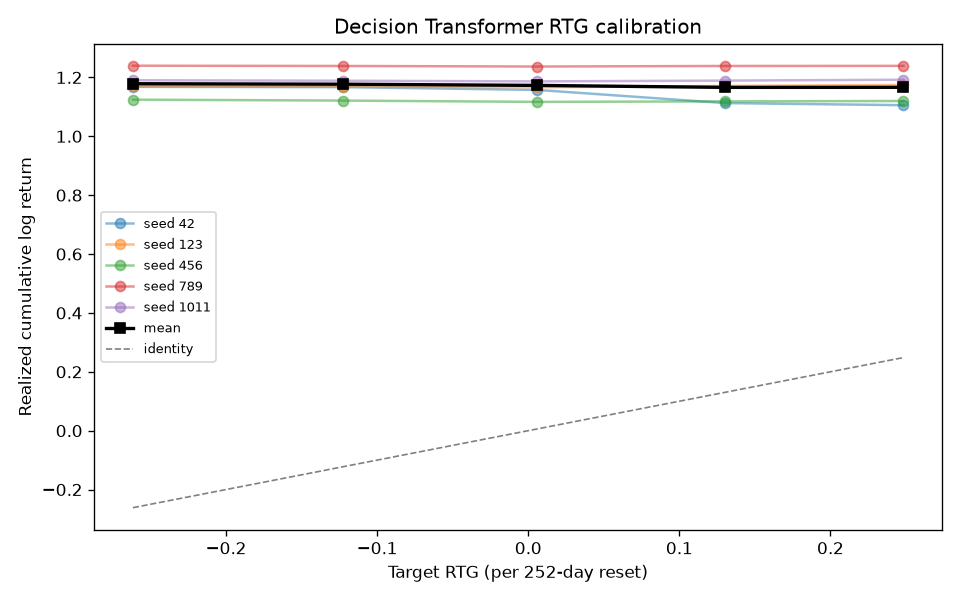
\includegraphics[width=0.92\textwidth]{rtg_calibration.png}
\caption{RTG calibration: target quantile versus realized log return.}
\end{figure}

\paragraph{Why RTG is unused.}
(1)~MSE clones $\mathcal{D}$ and never \emph{rewards} changing $a$ with $\hat R$.
(2)~$\sigma_{\mathrm{RTG}}$ is small ($\sim$0.14 log-return per 252-day episode)
while the test path is $\sim$1{,}500 days.
(3)~Resetting every 252 days severs a six-year target.
DT therefore behaves like a slightly noisier BC.

\subsection{Transformer BC}

File: \path{src/models/bc.py} \texttt{TransformerBC}.

\paragraph{Math.}
Same GPT, tokens $(s_t,a_t)$ only (2 tokens/day, state at even indices
\texttt{x[:, 0::2]}). Same last-step MSE, \textbf{no RTG}.

\paragraph{Why it exists.}
Ablation of return conditioning. If DT $\approx$ BC, RTG is not doing work.

\paragraph{Result.}
CAGR $21.9\%$, Sharpe $0.976\pm 0.095$.
Tightest learned clone of the behavior mixture; the correct control for DT.
Slightly \emph{better} than DT on mean Sharpe (overlapping seed ranges).

\texttt{MLPBC} is implemented but \textbf{not} in the 8-model sweep.

\section{Offline RL algorithms}
\label{sec:offline}

File: \path{src/models/offline_rl.py}.
All use \texttt{last\_state\_only} batches: $(s,a,r,s',d)$ with genuine next
states and \texttt{dones} at episode ends.
Actors: \texttt{SimplexActor} (MLP $2580\to 256\to 256\to 14$, softmax).
Critics: twin $Q(s,a)$ MLPs.
Polyak $\tau=0.005$, $\gamma=0.99$, Adam $3\times 10^{-4}$.

\paragraph{Bugs that had to be fixed before the sweep}
(or the table is fiction): $s'=s$ (self-Bellman), frozen target nets,
CQL \texttt{logsumexp} over the \emph{batch}, IQL $V$ chasing live $Q$,
checkpoints saving the algorithm \emph{name}.
Covered by \path{tests/test_training_regressions.py}.

\subsection{TD3+BC}

\paragraph{Math.}
Twin delayed DDPG + a BC tether (Fujimoto \& Gu):
\begin{align}
y &= r+\gamma(1-d)\min_{i=1,2}Q_{\theta'_i}(s',\pi_\phi(s')), \\
\mathcal{L}_Q &= \sum_{i=1}^2\|Q_{\theta_i}(s,a)-y\|_2^2, \\
\mathcal{L}_\pi &= -\alpha\,\mathbb{E}[Q_{\theta_1}(s,\pi_\phi(s))]
+\|\pi_\phi(s)-a_{\mathrm{data}}\|_2^2,
\end{align}
with $\alpha=2.5$, $\theta'\leftarrow(1-\tau)\theta'+\tau\theta$.

\paragraph{Implementation notes.}
No target \emph{actor} and no target-action noise (simplex + softmax).
\texttt{alpha} multiplies $Q$; it is not the usual $\lambda$ that scales BC
by $|Q|$.

\paragraph{Result.}
Weakest serious offline agent: Sharpe $0.66\pm 0.23$, CAGR $19.0\%$,
DD $-35\%$.
BC term plus a high-dimensional state is not enough to beat $1/N$;
seed variance is large.

\subsection{IQL (Implicit Q-Learning)}

\paragraph{Math.}
Fit $V$ with expectile $\tau_e=0.7$ to a \emph{frozen} target $Q$, then TD
on $Q$ using $V(s')$, then advantage-weighted BC:
\begin{align}
\mathcal{L}_V &= \mathbb{E}\bigl[|\tau_e-\mathbf{1}_{Q-V<0}|
(Q_{\theta'}(s,a)-V_\psi(s))^2\bigr], \\
y &= r+\gamma(1-d)V_\psi(s'),\qquad
\mathcal{L}_Q=\sum_i\|Q_{\theta_i}(s,a)-y\|_2^2, \\
\mathcal{L}_\pi &= \mathbb{E}\bigl[e^{\mathrm{clip}((Q-V)/T,\,100)}\,
\|\pi(s)-a\|_2^2\bigr],\quad T=3.
\end{align}

\paragraph{Why a target $Q$.}
Fitting $V$ to live $Q$ is the deadly triad; loss went to $10^4$.
After Polyak, value loss is $\sim 5\times 10^{-4}$.

\paragraph{Result.}
Sharpe $0.82\pm 0.18$, CAGR $19.6\%$.
Conservative (expectile + AWR) and below BC: it down-weights the high-return,
high-turnover trajectories in $\mathcal{D}$ instead of beating $1/N$.

\subsection{CQL (Conservative Q-Learning)}

\paragraph{Math.}
TD plus a CQL(H) penalty over $N_a=10$ random simplex actions
$\tilde a\sim\mathrm{softmax}(\mathcal{N})$, $\alpha_{\mathrm{CQL}}=1$:
\begin{align}
\mathcal{L}_Q &= \mathrm{TD}
+\alpha_{\mathrm{CQL}}\sum_{i=1}^2\Bigl(
\log\sum_{j=1}^{N_a}e^{Q_{\theta_i}(s,\tilde a_j)}
-\mathbb{E}_{a\sim\mathcal{D}}[Q_{\theta_i}(s,a)]\Bigr), \\
\mathcal{L}_\pi &= -\mathbb{E}[Q_{\theta_1}(s,\pi(s))]
+\|\pi(s)-a_{\mathrm{data}}\|_2^2.
\end{align}

\paragraph{Implementation trap.}
\texttt{logsumexp} over the \textbf{batch} is $\approx 2\log B$ and does not
penalize OOD actions. The code logsumexps over the action-sample axis.
The actor has a BC anchor so $-\,Q$ cannot drift to $-16$.

\paragraph{Result.}
Highest CAGR $34.3\%$ but Sharpe only $0.78\pm 0.19$, vol $34.6\%$,
max DD $-50\%$.
Seed 789 alone has $53\%$ CAGR --- a risk-on outlier, not a stable Sharpe engine.
Walk-forward: $0.19$ / $0.95$ / $-0.02$ / $1.44$.
CQL \emph{does} leave the data support (that is the point of $-\,Q$) and pays
for it in drawdown.

\section{``Online'' reference algorithms}
\label{sec:online}

File: \path{src/models/online_rl.py}.
\textbf{Not true online RL.} They take one gradient step per offline batch.
Treat as extra imitation/Q variants, not as an online upper bound.

Dirichlet actor (PPO, SAC): $\alpha=\mathrm{softplus}(f(s))+1$, then
\texttt{nan\_to\_num} and clamp (guards the old NaN).
Inference uses $\mathbb{E}[\mathrm{Dir}(\alpha)]=\alpha/\|\alpha\|_1$.

\subsection{PPO (simplified)}

\paragraph{Intended math.}
Clipped surrogate on $\rho_t=\pi/\pi_{\mathrm{old}}$.

\paragraph{What the code actually does.}
\begin{lstlisting}
ratio = exp(log_prob - log_prob.detach())   # = 1 identically
\end{lstlisting}
So the clip never fires. Advantage is $r-V(s)$ with \textbf{no GAE, no bootstrap
from $s'$}. Critic fits $V\to r$ (one-step reward, not return).
This is closer to a broken one-step A2C than to PPO.

\paragraph{Result.}
Sharpe $1.118$, std $0$, identical to buy-and-hold on \textbf{every seed}.
The Dirichlet mean collapsed to uniform.
It ``wins'' among learned methods by copying $1/N$, not by allocating.

\subsection{SAC (simplified)}

\paragraph{Intended math.}
Soft $Q$ with entropy $\alpha\log\pi$.

\paragraph{What the code actually does.}
One critic (not twins). Target $r+\gamma(1-d)Q(s',\pi(s'))$.
Actor $\mathcal{L}=-\mathbb{E}[Q(s,\pi(s))]$ --- entropy weight
\texttt{self.alpha} is unused. Dirichlet sample/mean for $\pi(s)$.

\paragraph{Result.}
Best \emph{non-collapsed} learned Sharpe: $1.039\pm 0.143$, CAGR $22.2\%$,
still below $1/N$. Mild turnover ($5.8\%$).
Closest learned policy to the baseline besides PPO.

\subsection{A2C}

\paragraph{Math (implemented).}
Softmax actor, $A=r-V(s)$,
\begin{equation}
\mathcal{L}_\pi=-\mathbb{E}\bigl[A\cdot a_{\mathrm{data}}^\top\log\pi(s)\bigr],
\qquad
\mathcal{L}_V=\|V(s)-r\|_2^2.
\end{equation}
That is a cross-entropy toward \textbf{dataset} actions weighted by advantage,
not a sampled on-policy A2C.

\paragraph{Result.}
Broken as a portfolio: CAGR $-1.4\%$, Sharpe $-0.13\pm 0.34$,
turnover $>1$ per day (rebalancing the whole book constantly).
Ignore for allocation; keep only as a ``this interface can train'' check.

\section{Reading results across algorithms}
\label{sec:results}

\begin{figure}[ht]
\centering

\includegraphics[width=0.92\textwidth]{walkforward_sharpe.png}
\caption{Walk-forward Sharpe (classical heatmap from
\texttt{walkforward\_metrics.csv}).}
\end{figure}

Out-of-sample folds (learned $=$ mean over seeds):

\begin{center}
\begin{tabular}{lrrrrrr}
\toprule
Fold & BAH & Mom.\ & DT & BC & SAC & CQL \\
\midrule
2018--19 & 0.80 & 0.86 & 0.79 & 0.78 & 0.79 & 0.19 \\
2020--21 & 1.24 & 1.32 & 1.07 & 1.06 & 1.09 & 0.95 \\
2022--23 & 0.33 & 0.07 & 0.25 & 0.28 & 0.33 & $-0.02$ \\
2024--25 & 1.94 & 1.38 & 1.84 & 1.85 & 1.87 & 1.44 \\
\bottomrule
\end{tabular}
\end{center}

Learned curves \textbf{track} buy-and-hold and never lead.
2014--2017 folds overlap training (\texttt{in\_sample=True}) and are not
performance.

\paragraph{Statistics.}
Circular block bootstrap (block 20, 1{,}000 reps) and Ledoit--Wolf vs.\
buy-and-hold in \path{src/eval/stats.py}.
Deflated Sharpe uses $n_{\mathrm{trials}}=46$ (every classical row
\textbf{and} every seed), which drives DSR $\approx 0$ for everyone, including
BAH --- too conservative to be useful.

\paragraph{Mental model.}
\begin{lstlisting}
1/N  (BAH = EW = PPO-collapsed)
  ^ SAC slightly below
  ^ BC ~ DT  (sequence clone of D, RTG off)
  ^ IQL, TD3+BC  (conservative / weak)
  ^ CQL  (high CAGR, ugly risk)
  ^ Momentum  (high CAGR, high turnover)
  v Risk parity, A2C
\end{lstlisting}

\section{Inference path (how tables get filled)}
\label{sec:inference}

\begin{enumerate}
\item \texttt{training\_manifest.json} lists \texttt{dt\_seed42} $\to$
      checkpoint path; skip \texttt{failed:}.
\item \textbf{DT/BC:} \texttt{DTPolicy} keeps a rolling $K$ buffer, decrements
      RTG from \texttt{env.history[-1]["reward"]}, resets every 252 steps.
\item \textbf{RL:} \texttt{AgentPolicy} loads \texttt{modules},
      \texttt{get\_action}, \texttt{project\_to\_simplex}.
\item \texttt{backtest\_policy} $\to$ \texttt{PortfolioEnv.run\_policy} $\to$
      metrics in \path{src/eval/metrics.py}.
\item Means over seeds $\to$ \texttt{headline\_test\_metrics.csv} /
      \texttt{learned\_test\_metrics.csv}.
\end{enumerate}

\section{Challenges (short)}
\label{sec:challenges}

Documented at length in the paper \S Challenges. For study, the load-bearing
ones are:
\begin{enumerate}
\item \textbf{Exogenous + costs} $\Rightarrow$ turnover needs real edge;
      $1/N$ already has Sharpe $1.12$.
\item \textbf{RTG unused} $\Rightarrow$ DT is BC with extra tokens.
\item \textbf{RL correctness} $\Rightarrow$ always check $s'$, target nets,
      and what \texttt{logsumexp} is over.
\item \textbf{PPO/SAC/A2C} are not textbook algorithms here
      (ratio $=1$, unused entropy, offline batches).
\item \textbf{Hardware} forced 200 steps/epoch and no AMP.
\item \textbf{BAH $=$ EW} is an artifact of target-based turnover.
\end{enumerate}

\section{Where to read next}
\label{sec:next}

\begin{center}
\begin{tabular}{@{}ll@{}}
\toprule
Topic & File \\
\midrule
Paper & \path{paper/main.tex} \\
Hyperparameters & \path{configs/config.yaml} \\
Env / reward & \path{src/env.py} \\
Classical policies & \path{src/policies.py} \\
DT / BC & \path{src/models/decision_transformer.py}, \path{src/models/bc.py} \\
Offline / online RL & \path{src/models/offline_rl.py}, \path{src/models/online_rl.py} \\
Train / eval & \path{src/trainer.py}, \path{src/eval/} \\
Numbers & \path{results/tables/} \\
\bottomrule
\end{tabular}
\end{center}

\end{document}
